\chapter{Proceso de software ejecutado}\label{Proceso de software ejecutado}
%Función que crea el título de capítulo y al cual se le da el nombre deseado a través de su parámetro obligatorio. Al no tener la función el “*” se escribirá también en el título del documento las palabras “Capítulo 1: …”. Además se indica, mediante la función “\label”, la correspondiente etiqueta que lleva asociada. La etiqueta sirve para que en caso de que luego se quiera hacer referencia al capítulo se haga llamando etiqueta tal que se escribiría “La información correspondiente a dicho tema se encuentra en el capítulo \ref{Int}.”

\thispagestyle{fancy}
%Función que determina que durante este capítulo se aplique el estilo Fancy.

\fancyhead[LE]{\thechapter.Proceso de software ejecutado} 
%Función que se utiliza para indicar que en las páginas impares, aparezca en el encabezado en la parte izquierda, el número del capítulo con su correspondiente nombre.

En este capítulo, se van a explorar los requisitos del proyecto, el diseño seguido para cumplirlo, el desarrollo para poner en práctica la idea y por último la validación para comprobar su funcionamiento.

\section{Análisis}
Para poder resolver los problemas de identidad del mundo, hay que crear una lista de requisitos. Después de realizar el desarrollo, se volverá a visitar la lista para concluir si dicho desarrollo ha sido satisfactorio.

\subsection{Requisitos (funcionales y no funcionales)}
Antes de comenzar a desarrollar la solución, hay que analizar las posibilidades y elegir las librerías correctas.

\begin{center}
    \begin{table}[h!]
        \begin{tabular}{|p{0.1\linewidth} | p{0.8\linewidth}|}
            \hline
             
            \textbf{O1} & \textbf{Diseño de un sistema de SSI distribuido.} \\
            \hline
            RF1         & La plataforma debe contar con una página web estática. \\
            \hline
            RF2         & La plataforma debe poder enviar datos en un medio distribuido. \\
            \hline
            RF3         & La plataforma debe comunicarse con una red \textit{blockchain}. \\
            \hline
            RF4         & La plataforma debe poder identificar usuarios en un mundo medio distribuido. \\
            \hline
            RF5         & La plataforma debe procesar peticiones de los usuarios en un medio distribuido. \\
            \hline
            RNF1        & La plataforma debe ser \textit{open source}. \\
            \hline
            RNF2        & La plataforma debe usar librerías \textit{open source}. \\
            \hline
        \end{tabular}
    \end{table}
\end{center}
\textbf{La plataforma debe contar con una página web estática.}\\
Para poder desplegar nuestra aplicación web en IPFS, necesitamos que nuestra página sea estática. Esto significa que no podemos generar nuestro HTML en un servidor.
\begin{center}
    \begin{table}[h!]
        \begin{tabular}{|p{0.15\linewidth} | p{0.75\linewidth}|}
            \hline
             
            \textbf{O1-RF1} & \textbf{La plataforma debe contar con una página web estática.} \\
            \hline
            S111            & Empaquetado de \textit{assets}. \\
            \hline
            S112            & Optimización de código. \\
            \hline
            S113            & \textit{Code splitting.} \\
            \hline
        \end{tabular}
    \end{table}
\end{center}
\begin{itemize}
    \item \textbf{S111}: la herramienta debe tener una opción para poder empaquetar HTML, JS y CSS en un solo fichero JS.
    \item \textbf{S112}: la herramienta debe optimizar nuestra aplicación para que tenga un mejor rendimiento.
    \item \textbf{S113}: la herramienta debe poder dividir nuestro \textit{payload} en diferentes ficheros para no tener que enviar un archivo excesivamente grande.
\end{itemize}
\textbf{La plataforma debe poder enviar datos en un medio distribuido.}\\
Ya que se quiere implementar un sistema de identidades distribuidas, será necesario un canal por el que poder comunicar a todos los usuarios.
\begin{center}
    \begin{table}[h!]
        \begin{tabular}{|p{0.15\linewidth} | p{0.75\linewidth}|}
            \hline
             
            \textbf{O1-RF2} & \textbf{La plataforma debe poder enviar datos en un medio distribuido.} \\
            \hline
            S121            & Capacidad de mutar datos. \\
            \hline
            S112            & Seguro. \\
            \hline
        \end{tabular}
    \end{table}
\end{center}
\begin{itemize}
    \item \textbf{S121}: la herramienta tiene que ser capaz de proporcionar las herramientas necesarias de mutar datos. Este paso es esencial para implementar una base de datos.
    \item \textbf{S122}: la herramienta tiene que poder asegurarnos que el transporte de los datos es seguro entre nodos para evitar la suplantación de identidad.
\end{itemize}
\textbf{La plataforma debe comunicarse con una red \textit{blockchain}.}\\
Para poder verificar que el usuario es quien dice ser, se necesita un medio que garantice la trazabilidad de las identidades sin revelar los datos personales de las mismas.
\begin{center}
    \begin{table}[h!]
        \begin{tabular}{|p{0.1\linewidth} | p{0.8\linewidth}|}
            \hline
             
            \textbf{O1-RF3} & \textbf{La plataforma debe comunicarse con una red \textit{blockchain}.} \\
            \hline
            S131            & Exponer un método de comunicación desde la interfaz. \\
            \hline
            S132            & Compatible con librerías de escucha a contratos. \\
            \hline
        \end{tabular}
    \end{table}
\end{center}
\begin{itemize}
    \item \textbf{S131}: la herramienta tiene que exponer un puerto de comunicación desde el que se pueda enviar y recibir información.
    \item \textbf{S132}: la herramienta tiene que ser compatible con librerías de escucha a contratos para poder responder a eventos que ocurran.
\end{itemize}
\textbf{La plataforma debe poder identificar usuarios en un medio distribuido.}\\
A fecha de publicación de este trabajo, la web todavía no dispone de un estándar para las identidades distribuidas. Aún así, existe una propuesta en proceso de ser aceptada \cite{web:did-spec}.
\begin{center}
    \begin{table}[h!]
        \begin{tabular}{|p{0.15\linewidth} | p{0.75\linewidth}|}
            \hline
             
            \textbf{O1-RF4} & \textbf{La plataforma debe poder identificar usuarios en un medio distribuido.} \\
            \hline
            S141            & Decodificar DID. \\
            \hline
            S142            & Codificar DID. \\
            \hline
        \end{tabular}
    \end{table}
\end{center}
\begin{itemize}
    \item \textbf{S141}: la herramienta debe ser capaz de decodificar los DID y obtener la información necesaria.
    \item \textbf{S142}: la herramienta debe ser capaz de codificar el DID del usuario accediendo a su cartera.
\end{itemize}
\textbf{La plataforma debe procesar peticiones de los usuarios en un medio distribuido.}\\
Al no disponer de un \textit{backend}, tenemos que diseñar una alternativa para conseguir la misma funcionalidad utilizando el mundo distribuido. En vez de usar un patrón de diseño \verb|REST|, se va a utilizar \verb|gRCP|. Esto se debe a que el \textit{backend} no dispone de datos que cuales pueda devolver. Solo podemos ejecutar funciones.
\begin{center}
    \begin{table}[h!]
        \begin{tabular}{|p{0.1\linewidth} | p{0.8\linewidth}|}
            \hline
            
            \textbf{O1-RF5} & \textbf{La plataforma debe procesar peticiones de los usuarios en un medio distribuido.} \\
            \hline
            S151            & Exponer funciones para ser llamadas por los usuarios. \\
            \hline
        \end{tabular}
    \end{table}
\end{center}
\begin{itemize}
    \item \textbf{S151}: siguiendo un patrón \verb|gRCP|, se expondrán funciones con las que se podrá llamar desde la aplicación.
\end{itemize}
\textbf{La plataforma debe ser \textit{open source}.}\\
Para asegurar un desarrollo ético de este proyecto, se desarrollará bajo una licencia open source. Más adelante se explicarán las implicaciones éticas de este proyecto.
\begin{center}
    \begin{table}[h!]
        \begin{tabular}{|p{0.15\linewidth} | p{0.75\linewidth}|}
            \hline
             
            \textbf{O1-RNF1} & \textbf{La plataforma debe ser \textit{open source}.} \\
            \hline
            S11N1            & Licencia \textit{open source}. \\
            \hline
        \end{tabular}
    \end{table}
\end{center}
\begin{itemize}
    \item \textbf{S11N1}: para asegurar que el proyecto y los próximos que avancen lo creado en este sean \textit{open source}, se usará una licencia que lo pueda asegurar. \textbf{GNU General Public License v3.0}.
    \begin{table}[h!]
        \centering
        \begin{tabular}{|c|c|c|}
            \hline
            Permissions         & Limitations   & Conditions \\
            \hline
            Commercial use      & Liability     & License and copyright notice \\
            \hline
            Modification        & Warranty      & State changes \\
            \hline
            Distribution        &               & Disclose source\\
            \hline
            Patent use          &               & Same license \\
            \hline
            Private use         &               & \\
            \hline
        \end{tabular}
        \cite{web:LICENSE}
    \end{table}
\end{itemize}
\textbf{La plataforma debe usar librerías open source.}\\
Este proyecto, al ser open source, utilizará multiples librerías, todas ellas de código abierto. De esa manera, cualquier fragmento de código puede ser verificado.
\begin{center}
    \begin{table}[h!]
        \begin{tabular}{|p{0.15\linewidth} | p{0.75\linewidth}|}
            \hline
             
            \textbf{O1-RNF2} & \textbf{La plataforma debe usar librerías \textit{open source}.} \\
            \hline
            S11N2            & Licencia \textit{open source}. \\
            \hline
        \end{tabular}
    \end{table}
\end{center}
\begin{itemize}
    \item \textbf{S12N1}: las librerías usadas deberán usar licencias de código abierto.
\end{itemize}
\noindent\rule{\textwidth}{0.4pt}
\begin{center}
    \begin{table}[h!]
        \begin{tabular}{|p{0.1\linewidth} | p{0.8\linewidth}|}
            \hline
             
            \textbf{O2} & \textbf{Desarrollo de un sistema de SSI distribuido.} \\
            \hline
            RF1     & La plataforma debe ejecutar un nodo IPFS. \\
            \hline
            RF2     & La plataforma debe contar con las \verb|APIs| necesarias para comunicarse con la cartera del usuario.\\
            \hline
            RF3     & La plataforma debe ejecutar una base de datos OrbitDB. \\
            \hline
        \end{tabular}
    \end{table}
\end{center}
\textbf{La plataforma debe ejecutar un nodo IPFS.}\\
Como la herramienta elegida ha sido IPFS, se necesitará asegurar su correcto funcionamiento.
\begin{center}
    \begin{table}[h!]
        \begin{tabular}{|p{0.15\linewidth} | p{0.75\linewidth}|}
            \hline
             
            \textbf{O2-RF1} & \textbf{La plataforma debe ejecutar un nodo IPFS.} \\
            \hline
            S211     & Configuración correcta con servidores Star. \\
            \hline
            S212     & Configuración correcta de OrbitDB. \\
            \hline
            S213     & Generar métodos para descargar datos y desencriptarlos. \\
            \hline
            S214     & Generar métodos para subir datos y encriptarlos. \\
            \hline
        \end{tabular}
    \end{table}
\end{center}
\begin{itemize}
    \item \textbf{S211}: de deberá configurar IPFS correctamente para que los usuarios se puedan encontrar entre ellos.
    \item \textbf{S212}: para que las bases de datos se puedan replicar correctamente, OrbitDB necesita estar configurado correctamente.
    \item \textbf{S213}: para poder subir información a IPFS, se necesitará que esté encriptada para la seguridad del usuario.
    \item \textbf{S214}: para descargar información de IPFS, se necesitará desencriptarlos.
\end{itemize}
\textbf{La plataforma debe contar con las APIs necesarias para comunicarse con la cartera del usuario.}\\
Para poder comunicarnos con la cartera necesitaremos utilizar el objeto \verb|window.ethereum| correctamente.
\begin{center}
    \begin{table}[h!]
        \begin{tabular}{|p{0.15\linewidth} | p{0.75\linewidth}|}
            \hline
             
            \textbf{O2-RF2} & \textbf{La plataforma debe contar con las APIs necesarias para comunicarse con la cartera del usuario.} \\
            \hline
            S221     & Métodos auxiliares para usar la funcionalidad de la cartera \\
            \hline
        \end{tabular}
    \end{table}
\end{center}
\begin{itemize}
    \item \textbf{S221}: se crearán métodos generalistas para poder comunicarse con Metamask.
\end{itemize}
\textbf{La plataforma debe ejecutar una base de datos OrbitDB.}\\
Para poder ejecutar una base de datos, se necesitará crear una instancia de IPFS.
\begin{center}
    \begin{table}[h!]
        \begin{tabular}{|p{0.15\linewidth} | p{0.75\linewidth}|}
            \hline
             
            \textbf{O2-RF3} & \textbf{La plataforma debe contar con las APIs necesarias para comunicarse con la cartera del usuario.} \\
            \hline
            S231     & Generar claves para la comunicación. \\
            \hline
            S232     & Generar base de datos \textit{keyvalue} (clave-valor). \\
            \hline
            S233     & Generar métodos de escucha de eventos. \\
            \hline
            S234     & Subir DID a la base de datos. \\
            \hline
        \end{tabular}
    \end{table}
\end{center}
\begin{itemize}
    \item \textbf{S231}: para poder iniciar la comunicación, se necesitará generar las claves pública y privada.
    \item \textbf{S232}: se necesitará crear una base de datos \textit{keyvalue}.
    \item \textbf{S233}: para poder avisar al usuario de lo que ocurra, hay que poder escuchar eventos en la red.
    \item \textbf{S234}: para presentar al usuario ante el resto, habrá que subir su identificación a la base de datos.
\end{itemize}
\section{Diseño}
En este apartado, se va a diseñar la solución para poder cumplir los requisitos del sistema.
\subsection{Arquitectura general}
\begin{figure}[h!]
    \centering
    \includegraphics[width=0.9\textwidth]{Figures/Diseño.png}
    \caption{Diseño de la aplicación. Los nodos color verde son puertos de escucha IPFS. El nodo de color naranja es un puerto de escucha de Metamask.}
\end{figure}
Este es el diseño actual de la solución. \textit{A priori}, parece imposible que pueda funcionar ya que no existe ningún tipo de \textit{backend} en el que podamos ejecutar la lógica. Toda la lógica se ejecuta utilizando \textit{smart contracts} y el resto son intercambios de datos por IPFS.
La conexión de Metamask con la \textit{blockchain} está fuera del área de control. Para poder interactuar con la cartera, se dispondrá de un canal de comunicación en el que se puede enviar mensajes.
\begin{lstlisting}
    const syncKey = await window.ethereum.request({
			method: '',
			params: [],
    });
\end{lstlisting}
Utilizando esta función, podemos enviar un \verb|method| y unos argumentos. Los métodos son las funcionalidades que puede hacer Metamask.
Por ejemplo, para poder compartir la identidad del usuario y empezar a trabajar, es necesario que pedirle permiso. 
\begin{lstlisting}
    let encryptionPublicKey;
    ethereum
    .request({
        method: 'eth_getEncryptionPublicKey',
        params: [account], 
        // you must have access to the specified account
    })
    .then((result) => {
        encryptionPublicKey = result;
    })
    .catch((error) => {
        if (error.code === 4001) {
        // EIP-1193 userRejectedRequest error
        console.log("We can't encrypt anything without the key.");
        } else {
        console.error(error);
        }
    });
\end{lstlisting}
\cite{web:Metamask_wiki}
\subsection{Modelo funcional}
A diferencia de otros \textit{frameworks} clásicos que utilizan el modelo MVC (Model, View, Controller), Next.js, aunque capaz de hacer renderizado por servidor, su función principal es generar páginas estáticas. Estas páginas, para ser renderizadas, son llamadas como una función. React, como ya se ha dicho antes, utiliza \verb|JSX| \cite{web:jsx}, siendo capaz de añadir HTML en JS.
\begin{lstlisting}
    import Header from '../components/header';
    import HeroSection from '../components/hero';
    import Head from 'next/head';

    export default function Home() {
        return (
            <>
                <Head>
                    <title>TFG self soverign identity</title>
                    <meta name="viewport" content="initial-scale=1.0, width=device-width" />
                </Head>
                <Header />
                <HeroSection />
            </>
        );
    }
\end{lstlisting}
Para poder renderizar la página inicial (index), se necesita ejecutar la función Home, que tiene un \verb|return|, que devuelve HTML.
Cuando un usuario solicita la página, se le devuelve el HTML ya generado con el archivo JS que ha creado ese HTML en el servidor a la hora de de construirlo. El navegador ejecuta ese archivo de JS \textit{hidratando} la página y añadiendo toda la funcionalidad.
\subsection{Escucha de eventos}
\begin{figure}[h!]
    \centering
    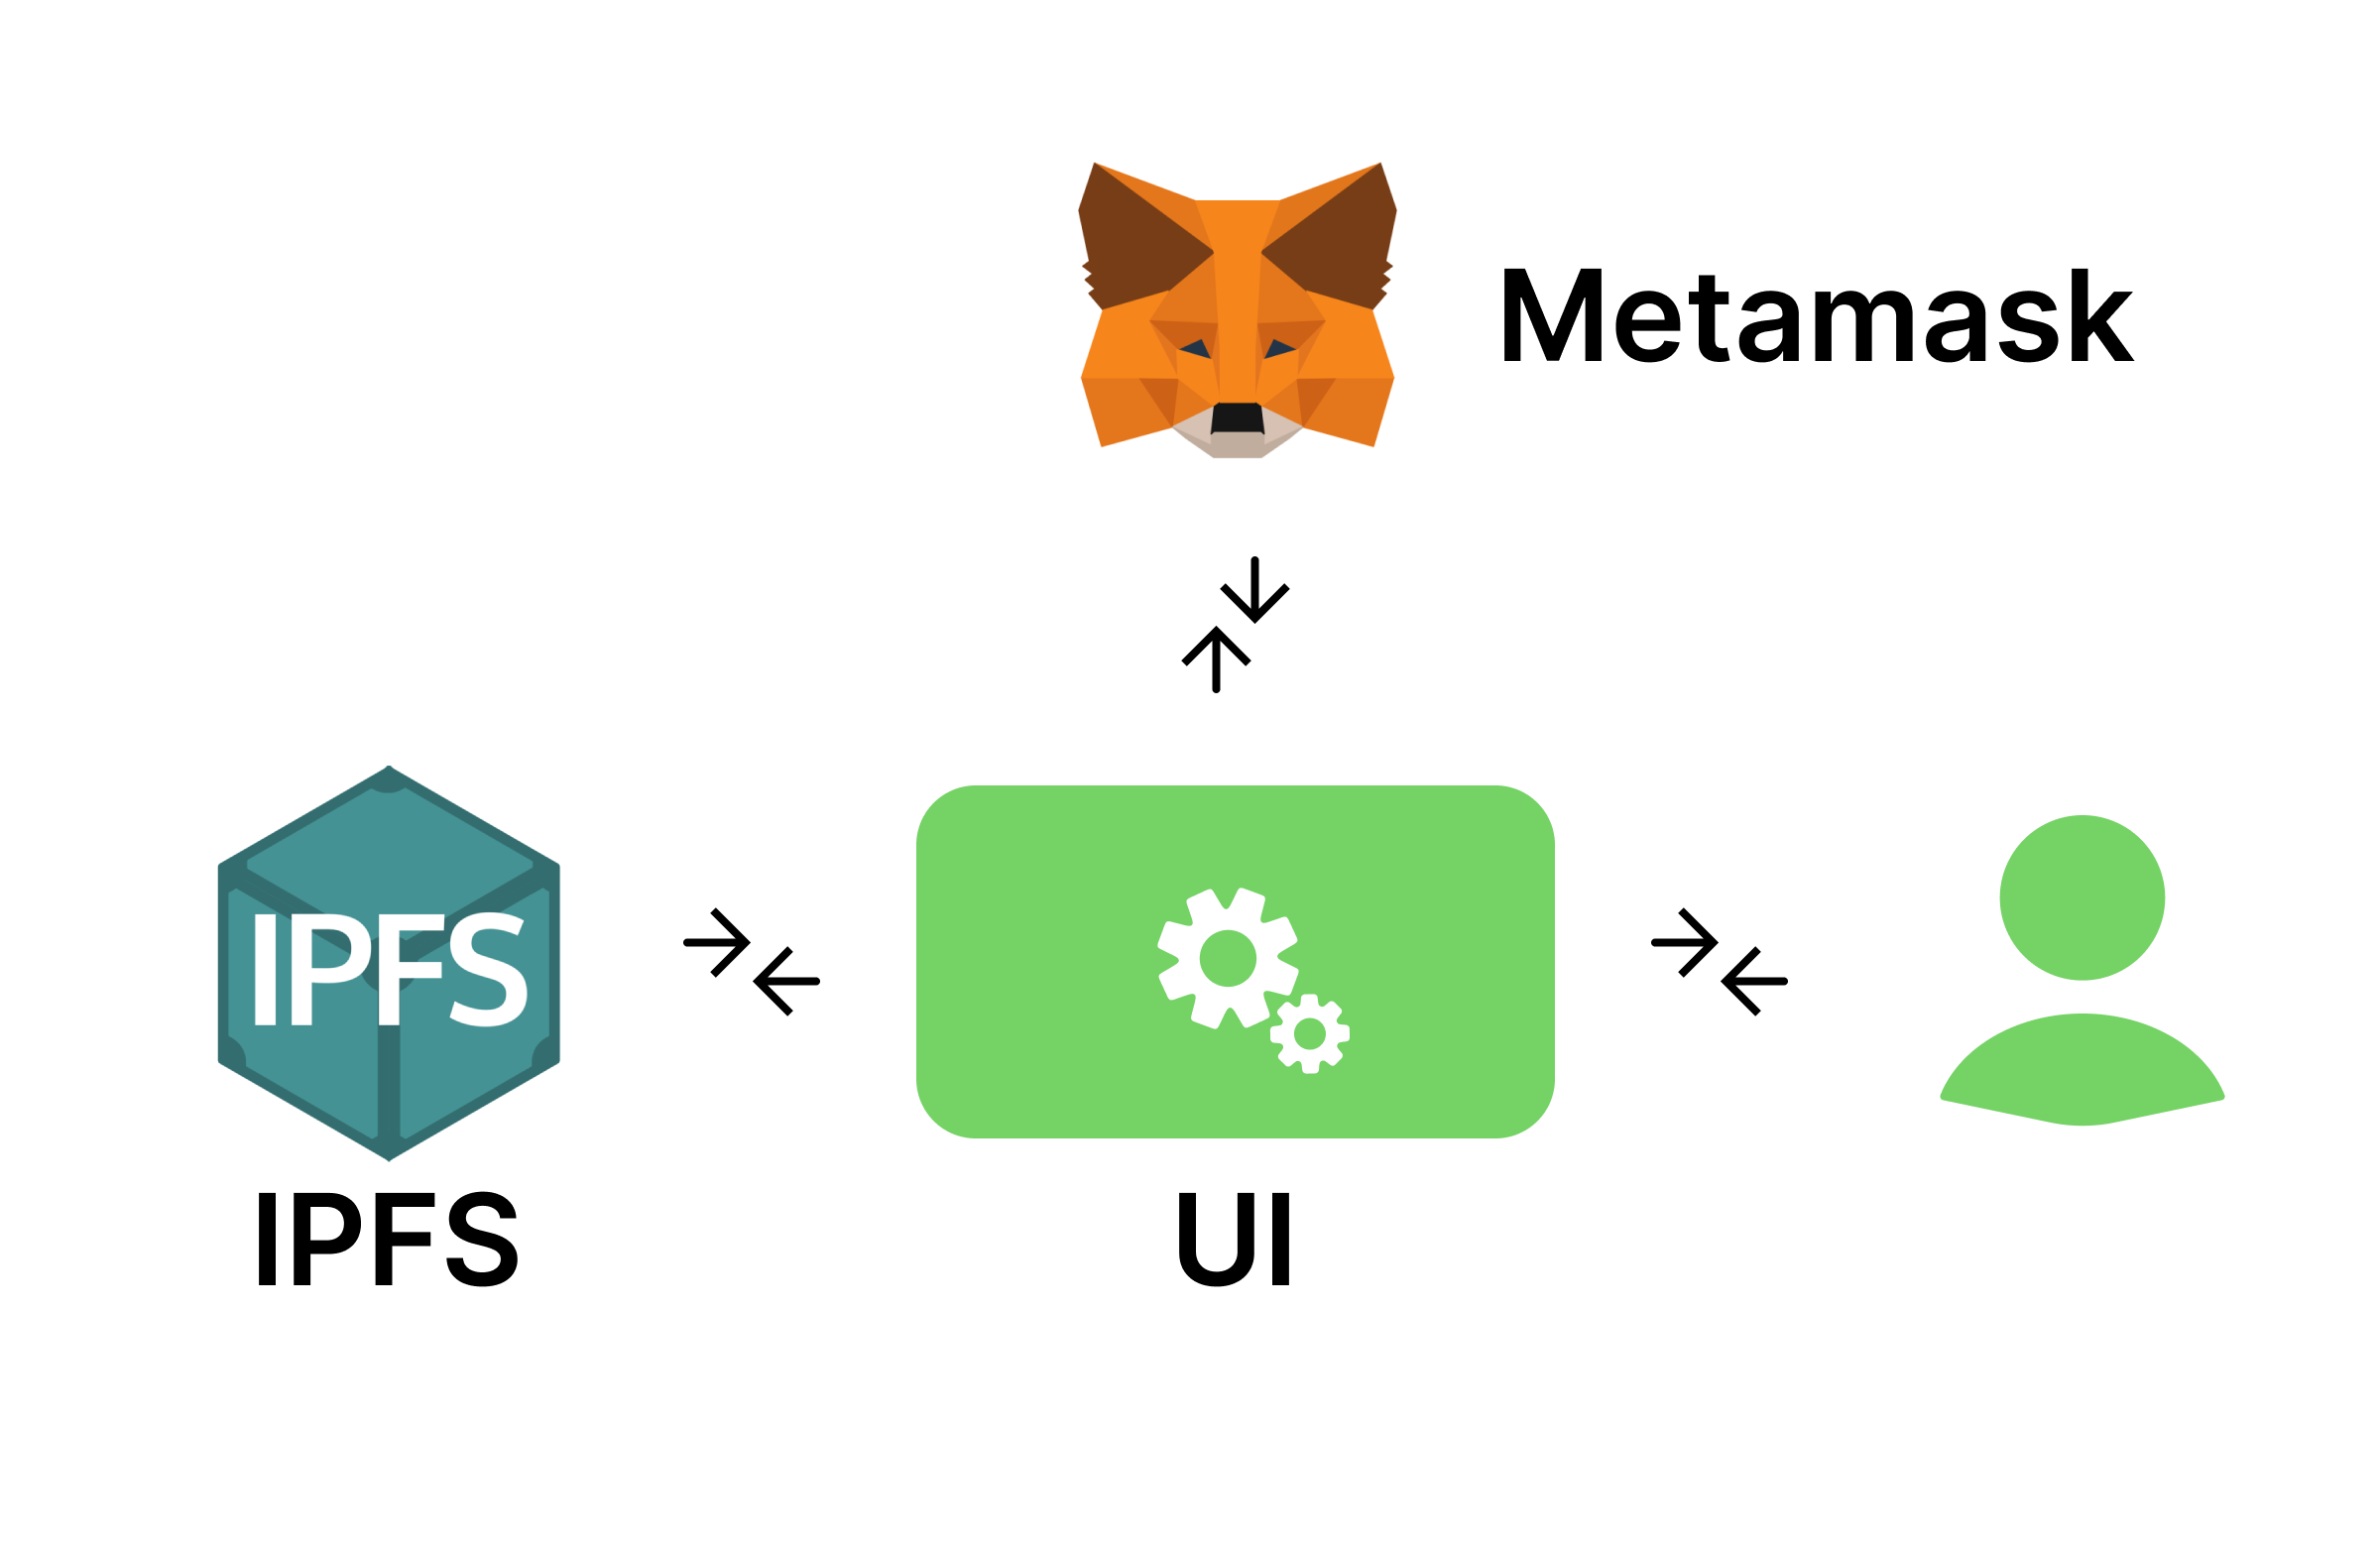
\includegraphics[width=0.9\textwidth]{Figures/Reactividad.png}
    \caption{Diagrama que muestra cómo la UI puede reaccionar a eventos que ocurren en la red para mostrar los cambios al usuario.}
\end{figure}
Este proyecto, una vez \textit{hidratado}, es capaz de escuchar eventos en la red. Gracias a esto, la UI es capaz de reaccionar y cambiar adecuadamente. Todo esto ocurriendo a tiempo real. Así mismo, también puede reaccionar a las acciones del usuario adecuadamente.
\subsection{Rutas}
Las rutas en Next.js no son programáticas sino contextuales. Las rutas se declaran creando archivos \verb|.js| en la carpeta pages.
\begin{lstlisting}
> tree
.
|-- _app.js
|-- index.js
|-- login.js
|-- upload.js

0 directories, 4 files
\end{lstlisting}
Este árbol explica que hay tres rutas más un fichero con funcionalidad especial.
\begin{itemize}
    \item \verb|index|
    \item \verb|login|
    \item \verb|upload|
\end{itemize}
El archivo \verb|_app| es un archivo que \textit{configura} al resto de las rutas.
Como el método de \verb|index| se llama \verb|Home|, el JSX resultante quedaría así.
\begin{lstlisting}
    <App>
        <Home/>
    </App>
\end{lstlisting}
En el método \verb|App|, podemos introducir lógica para que se ejecute en cada página, incluyendo también el HTML indicado en cada una. En este lugar, se puede establecer la lógica necesaria para comunicarse con la cartera del usuario y una manera para poder compartir el estado global a lo largo de toda la aplicación.
De este modo, al tratarse de una SPA \cite{web:spa} (Single page application), podemos mantener esa conexión y guardar por ejemplo la dirección del usuario o la conexión IPFS.
\newpage
\subsection{Diseño final}
\begin{figure}[H]
    \centering
    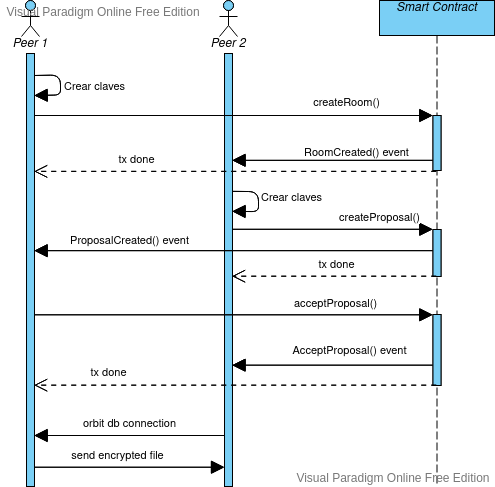
\includegraphics[width=0.8\textwidth]{Figures/Secuencia 1.png}
    \caption{Diagrama de secuencia de la aplicación.}
\end{figure}
\newpage
\section{Desarrollo}
En este punto, se va a exponer el desarrollo del proyecto siguiendo las guías establecidas en la sección de diseño.
\subsection{Entorno de desarrollo}
El entorno elegido para el desarrollo, es un ordenador fijo con un sistema operativo UNIX-like \cite{web:unix-like}, con la última version de Node.js instalada. Este sistema operativo ha sido escogido por varios motivos. Al ser un sistema operativo centrado en la consola la experiencia de desarrollo, es muy superior a la que Windows puede ofrecer. Así mismo, al ser un sistema operativo de código abierto, concuerda con la filosofía de este proyecto.
El navegador principal en el que se han realizado todas las pruebas ha sido Firefox, también de código abierto.
Este sistema operativo, en especifico, Arch Linux \cite{web:arch}, era conocido, por lo tanto se pudo comenzar a diseñar de inmediato.
Como administrador de paquetes, en vez de utilizar \verb|npm| \cite{web:npm}, se decidió elegir \verb|yarn| \cite{web:yarn} ya que consigue instalar los paquetes a una velocidad superior permitiendo alcanzar una calidad de desarrollo elevada. \verb|yarn|, como \verb|npm|, es un gestor de paquetes que lee el contenido de \verb|package.json| y descarga todas las dependencias en \verb|node_modules|.
\begin{lstlisting}
    "dependencies": {
	"@ethersproject/providers": "^5.5.3",
    "@Metamask/eth-sig-util": "^4.0.0",
    "@web3-react/core": "^6.1.9",
    "@web3-react/injected-connector": "^6.0.7",
    "@web3-react/walletconnect-connector": "^6.2.10",
    "axios": "^0.26.1",
    "bcrypt": "^5.0.1",
    "eth-crypto": "^2.2.0",
    "ethereumjs-util": "^7.1.4",
    "ethr-did": "^2.2.0",
    "ethr-did-resolver": "^5.0.4",
    "file-saver": "^2.0.5",
    "ipfs": "^0.62.1",
    "next": "12.0.10",
    "orbit-db": "^0.28.3",
    "orbit-db-identity-provider": "^0.4.0",
    "react": "^17.0.2",
    "react-dom": "^17.0.2",
    "react-ipfs": "^0.3.1",
    "react-query": "^3.34.16",
    "secp256k1": "^4.0.3",
    "tweetnacl": "^1.0.3",
    "tweetnacl-util": "^0.15.1",
    "use-callback-ref": "^1.2.5",
    "uuid": "^8.3.2",
    "web3": "^1.7.0"
    },
    "devDependencies": {
    "autoprefixer": "^10.4.2",
    "concurrently": "^7.1.0",
    "eslint": "^8.9.0",
    "eslint-plugin-react": "^7.28.0",
    "postcss": "^8.4.6",
    "tailwindcss": "^3.0.22"
    }
\end{lstlisting}
Todas estas dependencias son descargadas y analizadas para realizar la instalación óptima.
Hay dos tipos de dependencias:
\begin{itemize}
    \item \textbf{Desarrollo}\\
    Las dependencias de desarrollo, son solo librerías que se van a utilizar para elaborar nuestra aplicación. Por ejemplo, \verb|eslint| \cite{web:eslint} es una librería que escanea el estilo de código e intenta \textit{indentarlo} de la manera configurada.
    Por ejemplo, en el siguiente fragmento de código, existe un error de tabulación.
    \begin{lstlisting}
        export default function MainButton({ text }) {
        return (
        <button>{text}</button>
        );
        }
    \end{lstlisting}
    En cambio, después de ejecutar eslint, el código pasa a tener una estructura correcta.
    \begin{lstlisting}
        export default function MainButton({ text }) {
            return (
                <button>{text}</button>
            );
        }
    \end{lstlisting}
    \item \textbf{Producción}\\
    Las librerías de producción, son las utilidades que se han ido mencionando hasta ahora. Todas ellas son importantes para el funcionamiento de esta aplicación.
\end{itemize}
\subsection{Aplicación web}
Como ya se ha indicado anteriormente, Next.js \cite{web:next.js} es el \textit{framework} que se va a utilizar para la realización de este proyecto.
Tiene la siguiente estructura.
\begin{lstlisting}
    > tree -I 'node_modules|docs'
    .
    |-- components
    |   |-- button
    |   |   |-- index.js
    |   |-- header
    |   |   |-- index.js
    |   |-- hero
    |   |   |-- index.js
    |   |-- seccondaryButton
    |   |   |-- index.js
    |   |-- uploadPlatform
    |       |-- index.js
    |-- context
    |   |-- index.js
    |-- contracts
    |   |-- _FileShareControl.sol
    |-- ganache
    |   |-- README.md
    |-- package.json
    |-- pages
    |   |-- _app.js
    |   |-- index.js
    |   |-- login.js
    |   |-- upload.js
    |-- postcss.config.js
    |-- README.md
    |-- tailwind.config.js
    |-- utils
    |   |-- consts.js
    |   |-- index.js
    |-- yarn.lock

    11 directories, 19 files
\end{lstlisting}
Esta configuración no es obligatoria en su totalidad. Los únicos campos obligatorios son los archivos \verb|.js| en el directorio \verb|pages|.
El resto de las carpetas son elegidas por su \textit{expresividad}.\\
\textbf{Carpeta components}\\
    Esta carpeta contiene los componentes utilizados para el funcionamiento.
    En otros \textit{frameworks}, utilizaríamos plantillas para poder crear vistas del modelo M\textbf{V}C. Este cambio de paradigma hace pensar en piezas reutilizables.
    \begin{figure}[H]
        \centering
        
\includegraphics[width=0.5\textwidth]{Figures/Example UI.png}
        \caption{Interfaz de ejemplo para explicar un \textit{framework} basado en componentes.}
        \label{fg:ui}
    \end{figure}
    Tomando de ejemplo esta interfaz \ref{fg:ui}, se aprecia el mismo botón repetido multiples veces. Seguramente ese botón tenga funcionalidad diferente. Algunos pueden actuar de \textit{link} y otros pueden mutar datos de la base de datos.
    Todo esto haría que sea necesario crear múltiples botones en HTML con funcionalidad éspecifica cada uno. En un sistema clásico MVC, la creación de funcionalidad para botones se convierte en una tarea complicada.
    En cambio, en \textit{framework} basado en componentes, resulta una experiencia superior y mucho más modular.
    \begin{lstlisting}
        function Bt({text, onClick}) {
            return <button className='bg-blue-500' onClick={onClick}>{text}</button>
        }

        export default function Hero({content}) {
            return (
                // ...
                {
                    content.forEach(row => {
                        <div className='flex justify-between gap-5 ...'>
                            <p>{row.content}</p>
                            <Bt text={row.action.text} onClick={row.action.action} />
                        </div>
                    })
                }
                // ...
            )
        }
    \end{lstlisting}
    Con este pequeño segmento de código, podemos generar una interfaz igual de funcional que un \textit{framework} MVC pero con renderizado en cliente. Sin necesidad de tener un \textit{backend} para leer una base de datos. Así mismo, nuestro controlador es el mismo navegador. Este interactúa con la \textit{blockchain} y con IPFS a demanda del usuario.
\subsection{Contexto}
El contexto de nuestra aplicación, es un grupo de variables globales. Hay dos tipos de variables que se usan en este proyecto.
Las variables asíncronas y las síncronas.
\begin{itemize}
    \item Las variables asíncronas exponen dos variables en un \textit{array}. La primera es el propio valor establecido y la segunda es una función que sirve para guardar el estado. Cuando se llama a la función para cambiar el estado, se avisa a React para actualizar la interfaz. Es muy parecido al \textit{Data-driven rendering} \cite{web:ddr} de los videojuegos. Son variables a las que no se les espera que cambien el estado para continuar con su ejecución. Esto implica que si se tiene que usar ese valor actualizado, se pueden tener condiciones de carrera \cite{web:race}.
    \begin{lstlisting}
        const [valor, introducirValor] = useState(1)
        //...
        console.log(valor)
        // 1
        introducirValor(2)
        console.log(valor)
        // 1 (stale)
    \end{lstlisting}
    Como se puede ver en este ejemplo, aunque hemos actualizado el valor, se sigue obteniendo el resultado incorrecto.
    \item Las variables síncronas, tienen disponible su valor nada más ser asignadas. Así mismo, estas variables no provocan un renderizado. Se comportan de una manera muy parecida a las variables clásicas de JavaScript.
    \begin{lstlisting}
        let valor = 1
        console.log(valor)
        // 1
        valor = 2
        console.log(valor)
        // 2
    \end{lstlisting}
    En React, utilizamos un \textit{hook} para mejorar la experiencia de desarrollo. Aunque, a nivel práctico, su funcionamiento es idéntico.
    \begin{lstlisting}
        const valor = useRef(1)
        //...
        console.log(valor.current)
        // 1
        valor.current = 2
        console.log(valor.current)
        // 2
    \end{lstlisting}
    El nombre de la variable viene continuado por \verb|.current|. Esto se explicará mas adelante.
\end{itemize}
\subsection{Base de datos}
Este proyecto difiere de todos los paradigmas actuales introduciendo una base de datos distribuida. Esta base de datos se parece mucho a la \textit{blockchain}, ya que todo el mundo tiene una copia de los datos que contiene. Por ahora no existe una adaptación de una base de datos tipo relacional \cite{web:relational-database}; Solo existen los siguientes tipos:
\begin{itemize}
    \item \textbf{Log}\\
    Un registro de solo entrada con la capacidad de explorar el historial. Útil cuando se quiere saber la ultima entrada.
    \item \textbf{Feed}\\
    A diferencia del anterior, en este tipo de base de datos sí que se pueden mutar los datos. Es útil para un uso parecido a un carrito de la compra.
    \item \textbf{Key Value}\\
    Este tipo de base de datos funciona exactamente igual que Redis \cite{web:redis}. También se puede  comparar con el funcionamiento de un \textit{Hash map} \cite{web:hash-table}.
    \item \textbf{Docs} \\
    Implementación minima de una base de datos documental. Los archivos se consideran documentos a los cuales se puede acceder por su nombre. Parecido a MongoDB \cite{web:mongodb}, pero más limitado.
    \item \textbf{Counter} \\
    Útil para contar eventos de manera separada al Log o al Feed.
\end{itemize}
\subsection{Key Value}
La base de datos utilizada para este proyecto ha sido la \textbf{key value} ya que se pueden asignar datos a direcciones de la cartera de cada usuario.
En el mundo distribuido, cada persona tiene su base de datos, pero es dependiente del dominio al que pertenece. Eso quiere decir que si viene un usuario nuevo, hay que generar su DID \cite{web:did}.
Para poder comenzar a compartir información, hay que conectarse o crear una base de datos. Como se ha dicho anteriormente, todos los conectados a una base de datos comparten la misma información. Eso significa que a niveles prácticos todos los usuarios que estén conectados entre sí en la misma sala compartirán dirección entre ellos.
Las salas son las propias aplicaciones. Una sala puede ser desde Alud a un Twitter descentralizado.
Como estamos todos conectados, si el usuario \textbf{0xc0ffee254729296a45a3885639AC7E10F9d549} quiere obtener la clave pública del usuario \textbf{0x70E3Aed5aA1aac6EC39D114B7411DF6f1CC80671}, simplemente tiene que buscar su entrada en la base de datos.
\subsection{Permisos}
Para poder entrar a una sala se necesitan permisos. Por la misma razón que actualmente se necesita un usuario y contraseña para entrar en la mayoría de las paginas de internet, en el mundo distribuido ocurre lo mismo.
Cuando se crea una base de datos se pueden asignar dos tipos de permisos:
\begin{itemize}
    \item \textbf{Público}\\
    A la hora de generar la base de datos se puede especificar un ``*''. Esto significa que cualquier identificador puede escribir.
    \begin{lstlisting}
        let options = {
			// Give write access to yourself at first
			accessController: {
				write: [
					*,
				],
			},
		};
    \end{lstlisting}
    \item \textbf{Privado}\\
    Para la aplicación y generalmente para cualquier uso serio de esta tecnología, las bases de datos deben ser permisionadas.
    \begin{lstlisting}
        let options = {
			// Give write access to yourself at first
			accessController: {
				write: [
					OrbitDB.identity.id,
				],
			},
		};
    \end{lstlisting}
\end{itemize}
El objeto \verb|OrbitDB.identity.id|, es el identificador del creador. Es como la matricula de un coche. Un justificante criptográfico que permite la aceptación de mensajes dependiendo de si el origen es correcto o no. De este modo se evitan maneras de sobrescribir datos, como explicado en el capitulo de tecnologías utilizadas.
\subsection{Smart contract}
Para poder aceptar a personas en nuestra sala, necesitamos una forma de identificar a personas y verificar que son autenticas. Si implementamos una base de datos pública en la que cualquier persona puede introducir sus credenciales, alguien con peores intenciones puede sobrescribirlas consiguiendo robar información.
En cambio, introduciendo la tecnología \textit{blockchain}, se pueden utilizar todas sus posibilidades criptográficas para verificar que el origen es autentico. En esta aplicación, cualquier persona puede crear una sala y solicitar unirse a otra. Como la \textit{blockchain} es un registro total de todas las transacciones, siempre existe un registro de qué salas han sido creadas y si alguien ha querido entrar mientras no se estaba escuchando.
\begin{lstlisting}
// SPDX-License-Identifier: GPL-3.0

pragma solidity >=0.7.0 <0.9.0;

/**
 * @title FileShareControl
 * @dev Publish and allow users into your db
 */
contract FileShareControl {
    struct Room {
        address owner;
        string orbit_db_url;
    }
    mapping (address => Room) rooms;
    // TODO: Use mapping for better use
    struct Proposal {
        address proposer;
        address proposalTo;
        string orbit_db_identity;
        bool accepted;
    }
    mapping (address => Proposal) proposals;

    // Declare events. Will be used in js 
    event RoomCreated(address owner, string url);
    event ProposalCreated(address owner, address proposer, string identity);
    event ProposalAccepted(address proposer, string url);

    function createRoom(string memory url) 
    public 
    {
        // We cannot use "rooms[address] = Room(0x00000...0, "...")"
        // because the right hand side creates a memory-struct "Room" that contains a mapping
        Room storage r      = rooms[msg.sender];
        r.owner             = msg.sender;
        r.orbit_db_url      = url;
        emit RoomCreated(msg.sender, url);
    }

    function createProposal(address proposalTo, string memory identity)
        public
    {
        Proposal storage p  = proposals[msg.sender];
        p.proposer          = msg.sender;
        p.proposalTo        = proposalTo;
        p.orbit_db_identity = identity;
        emit ProposalCreated(proposalTo, msg.sender, identity);
    }

    function acceptProposal(address proposer) 
    public 
    {
        // First get the origin room
        Room memory r = rooms[msg.sender];
        // Check if the room exists. If not, the struct is generated with default values.
        // Default value of address
        require(r.owner != 0x0000000000000000000000000000000000000000, "You don't have any room.");
        
        Proposal memory p = proposals[proposer];
        // Proposal checks
        require(p.proposer !=  0x0000000000000000000000000000000000000000 && p.proposalTo != 0x0000000000000000000000000000000000000000, "The proposal doesn't exists.");
        require(p.proposalTo == msg.sender, "You are not the origin");
        require(p.proposer == proposer, "(+_+)");
        require(!(p.accepted), "The proposal is already accepted");
        // Warn the proposer that he is accepted
        emit ProposalAccepted(proposer, r.orbit_db_url);
    }

}
\end{lstlisting}
El \textit{smart contract} se divide en tres métodos principales que son usados a la hora de verificación:
\begin{itemize}
    \item \verb|createRoom|: anuncia la creación de una sala para que el resto de la red sepa de su existencia.
    Esta sala tiene una URL que pertenece a la dirección de escucha de OrbitDB.
    \item \verb|createProposal|: crea una petición para entrar a una sala.
    Para poder entrar, hay que avisar al creador y adjuntar la identidad de OrbitDB para que se adjunte a la lista con permisos de escritura.
    \item \verb|acceptProposal|: acepta la solicitud. Este método es solo una manera de avisar correctamente al solicitante de que puede entrar. No muy útil cuando el usuario está conectado a la página directamente porque se podrían utilizar métodos tradicionales, sino porque al ser un registro histórico, también podría entrar en las siguientes ocasiones sin tener que quemar más gas.
\end{itemize}
\subsection{Eventos - OrbitDB y Ethereum}
Como ya se ha comentado anteriormente, nuestra interfaz tiene que ser capaz de reflejar a eventos de la red, tanto por parte de IPFS como por parte de Ethereum.
Las librerías web 3.0 nos ayudan a realizar esta tarea de una manera más eficaz. De todas formas, podemos encontrarnos con múltiples problemas:
la escucha de eventos se carga al inicio de la aplicación. Esto significa que la primera vez que JS \textit{hidrata} la página y es montado, se ejecutan nuestras funciones de escucha.
Para poder escuchar eventos generalmente se suelen usar las \textit{callbacks}. \textit{Callback} en español significa “llamada de vuelta”, es decir, que si ocurre algo avisará llamándonos de vuelta.
Esto se puede conseguir ya que JavaScript permite asignar como valor de una variable una función.
\begin{lstlisting}
    const functionInsideAvar = () => { return 1 + 1 }
\end{lstlisting}
Si se llama esta variable, nos devolverá la suma de \verb|1 + 1|, \verb|2|.
Esta función es relativamente \textit{inútil}, ya que no estamos aprovechando las posibilidades de los callbacks.
\begin{lstlisting}
    cosnt msghandler = (msg) => {console.log(msg)}

    msghandler('primero')
    msghandler('segundo')
\end{lstlisting}
Como se aprecia en este ejemplo, se puede pasar contenido a la función. Eso abre muchísimo las posibilidades. Estas funciones permiten que el \textit{framework} solo se preocupe de pasar los mensajes y dejar la lógica al desarrollador. Se necesitará desarrollar el procesamiento de los mensajes de Ethereum y los cambios en la base de datos de OrbitDB.
Con la librería \verb|web3-eth-contract|, se puede escuchar las transacciones de una cuenta en especifico:
\begin{quote}
    \verb|0x709f43F711A32498BFee2Be963dFc686aAD8B450|
\end{quote}
Como las interacciones son públicas, solo hay que escuchar la dirección indicada para obtener información útil. En esta dirección, vive el contrato en la \textit{blockchain} de desarrollo.
Cuando se compila el \textit{smart contract} con Remix, devuelve un archivo JSON con información para poder interactuar de manera mucho más sencilla con el contrato.
Al ser un archivo estático, también puede ser alojado en IPFS y \textit{pineado} en el nodo de desarrollo.
\begin{lstlisting}
    contract.current = new Contract(jsonInterface['abi'], ADDRESS);
\end{lstlisting}
\verb|jsonInterface| es el JSON que se lee desde IPFS. También hay que pasar como argumento la dirección de nuestro contrato, la cual es: \verb|0x709f43F71...AD8B450|.
Después de cargar el JSON, la librería ayuda a convertir direcciones y envíos de datos hexadecimales en funciones de js con tipos clásicos.
\begin{lstlisting}
    contract.current.events.RoomCreated(function(error, result) {
        if (error) {
            console.error(error);
            return;
        }
        if(result === null) {
            console.error('Result is null');
            return;
        }
        const returnValues = result.returnValues;
        const found = Object.keys(rooms).find((r) => returnValues.owner === r);
        if (found !== undefined) {
            rooms[returnValues.owner].url = returnValues.url;
        } else {
            rooms[returnValues.owner] = {
                owner: returnValues.owner,
                url: returnValues.url
            };
        }
        console.log('Room created event fired:', rooms);
        setRooms({...rooms});
    });
    contract.current.events.ProposalCreated(function(error, result) {
        if (error) {
            console.error(error);
            return;
        }
        if(result === null) {
            console.error('Result is null');
            return;
        }
        console.log('Proposal created event fired:', result);
        // Do the job
        // Check owner
        if(result.returnValues.owner !== account) return;
        // Check the presence in the array.
        const found = notifications.find(n => n.proposer === result.returnValues.proposer);
        // The data associated to the proposer will never change, so we don't need to update anything.
        if(found === undefined) {
            setNotifications([ ...notifications,{
                owner: result.returnValues.owner,
                proposer: result.returnValues.proposer,
                identity: result.returnValues.identity,
            }]);
        }
        
    });
    contract.current.events.ProposalAccepted(function(error, result) {
        if (error) console.log(error);
        if (result === null) {
            console.error('Result is null');
            return;
        }
        console.log('Proposal accepted event fired:', result);
        // Do the job
        if(result.returnValues.proposer === account) 
            handleConnectToPeerDatabase(result.returnValues.url);

    });
\end{lstlisting}
Por otra parte, OrbitDB, también nos expone eventos a los cuales se puede pasar \textit{callbacks}.
\begin{lstlisting}
    DB.current.events.on('ready', () => {
        setPeers({ ...DB.current.all });
    });
    // When database gets replicated with a peer, display results
    DB.current.events.on('replicated', () => {
        setPeers({ ...DB.current.all });
    });
    // When we update the database, display result
    DB.current.events.on('write', () => {
        setPeers({ ...DB.current.all });
    });
\end{lstlisting}
Los eventos importantes que vamos a utilizar son:
\begin{itemize}
    \item \verb|ready|
    \item \verb|replicated|
    \item \verb|write|
\end{itemize}
Después de que esos eventos se disparen se actualiza la interfaz con los datos de la base de datos.\\
\subsection{Tipos de variables}
\begin{itemize}
    \item \textbf{.current}\\ 
    Las variables que normalmente se llamarían DB y contract tienen un \verb|.current| de sufijo. Esto se debe a que es una variable síncrona. Este tipo de variable tiene un lugar concreto en memoria y es global e inmutable.
    Significa que no pueden ser sobrescritas ni duplicadas. Esto permite no encontrar con variables \textit{stale}. Como no se puede sobrescribir la variable hay que guardarlo en una variable interna.
    React ayuda con un \textit{hook} llamado \verb|useRef()|. Esto expone una variable estática, global e inmutable, mientras tiene una variable interna \verb|.current|, en la que se puede guardar lo que se necesite.
    \item \textbf{useState()}\\
    \verb|useState()| es otro \textit{hook} que aporta React. Este hook, devuelve un \textit{array} con un \textit{getter} y un \textit{setter}:
    \begin{lstlisting}
        const [ getter, setter ] = useState()
    \end{lstlisting}
    La primera variable es una manera de usar el valor que se tiene guardado en el \verb|useState()|. El segundo valor, es una función para poder actualizarlo. Llamar al \verb|setter('Nuevo valor')|, actualiza la UI y renderiza la página de nuevo.
    Esto aporta un nuevo problema, ya que el \textit{getter} se puede quedar \textit{stale}. Como no es una variable global, está anclada al momento de ejecución de la función. Esto significa que después de un \textit{rerender} las funciones que quieran acceder a los valores obtendrán los valores anteriores.\\
\end{itemize}
\subsection{Flujo de datos}
Finalmente, después de todo este desarrollo, los usuarios interactuarían con la página de la siguiente manera:
\begin{enumerate}
    \item \textbf{El usuario da permiso para tener acceso a su cartera y conocer su identidad.}\\
    Este paso es esencial para cumplir con los objetivos de este proyecto. Todos los pasos deben tener el permiso explícito del usuario. Cuando el usuario quiere iniciar sesión en la página, se le pedirá permiso; Verá esta ventana saliendo de su cartera. Él puede interactuar con esa ventana y la interfaz reaccionará a este evento.
    \begin{figure}[H]
        \centering
        \includegraphics[width=0.4\textwidth]{Figures/Metamask.png}
        \caption[Interfaz de Metamask]{Interfaz de Metamask cuando se pide permiso para conectar a una página. Wiki de Aragon. \cite{web:aragon}}
        \label{fg:aragon}
    \end{figure}
    Después de tener una conexión con su cartera \ref{fg:aragon}, se necesita una vez más su permiso. Como se ha comentado en el punto \textit{Introducción a la criptografía}, se necesita la clave pública de la cartera. Es con esta clave con la que se consigue encriptar y desencriptar la información.
    \begin{lstlisting}
    const publicKey = await window.ethereum
		.request({
			method: 'eth_getEncryptionPublicKey',
			params: [account]
	});
    \end{lstlisting}
    Se puede obtener de la siguiente forma, llamando al método \verb|eth_getEncryptionPublicKey|. Nuevamente, para recordar, Metamask vive \textit{fuera} de la \textit{burbuja de ejecución} del dominio. Esto significa que de manera literal se necesita pedir permiso para realizar cualquier operación con la cartera del usuario.
    \item \textbf{El usuario interactúa con una sala}
    \begin{itemize}
        \item \textbf{Crea la sala}\\
        Antes de crear esa sala, se necesitará generar las claves para definir la base de datos como una base de datos privada.
        \begin{lstlisting}
        const identity = await Identities.createIdentity(options);
        \end{lstlisting}
        Cuando ya se tiene la identidad que va a ser usada para el transporte y para los permisos de escritura, se puede empezar a crear la sala.
        Esta sala será \textbf{\textit{keyvalue}}.
        \begin{lstlisting}
        const db = await OrbitDB.keyvalue(account, options);
        await db.put(account, DID_safe);
        \end{lstlisting}
        Se sube el DID para que el resto de personas puedan verlo y enviar la información.
        Por último, solo queda contactar con el \textit{smart contract} con los métodos anteriormente vistos para poder avisar al resto de usuarios y actualizar la interfaz.
        \begin{lstlisting}
        contract.current.methods.createRoom(db.address.toString()).send({ from: account, gasPrice: '20000000000' });
        \end{lstlisting}
        A partir de este momento, otros usuarios pueden haber solicitado entrar en la sala. Gracias a los métodos de escucha se traduce en unas notificaciones en la interfaz del usuario.
        Si decide aceptar alguna de esas notificaciones, se ejecutarán las siguientes instrucciones.
        \begin{lstlisting}
        const jsonInterface = JSON.parse(identity);
        \end{lstlisting}
        Se lee la identidad que se obtiene del \textit{smart contract} y se \textit{parsea} con la clase JSON.
        \begin{lstlisting}
        await DB.current.access.grant('write', jsonInterface.id);
        \end{lstlisting}
        Finalmente se puede añadir al grupo de personas capaces de escribir en la base de datos.
        \begin{lstlisting}
        contract.current.methods.acceptProposal(proposer).send({ from: account, gasPrice: '20000000000' });
        \end{lstlisting}
        Lógicamente, solo queda avisar al solicitante que puede conectarse.
        \item \textbf{El usuario se une a una sala}\\
        Si el usuario desea unirse a una sala existente, la secuencia de ejecución es distinta.
        De la misma manera que si quiere crear una sala, se necesita generar las claves.
        \begin{lstlisting}
        const identity = await Identities.createIdentity(options);
        \end{lstlisting}
        Al no tener que iniciar la conexión por ahora, simplemente se actualiza la UI para avisar al usuario que tiene que esperar y se solicita al \textit{smart contract} la creación de una petición de entrada.
        \begin{lstlisting}
        contract.current.methods.createProposal(owner, JSON.stringify(identity)).send({ from: account, gasPrice: '20000000000' });
        \end{lstlisting}
        En algún momento, nuestra solicitud será aceptada y se podrá conectar a la base de datos.
        \begin{lstlisting}
        const db = await OrbitDB.open(url, {type: 'keyvalue'});
        \end{lstlisting}
            Abrimos la base de datos especificando la dirección obtenida desde el \textit{smart contract}.
        \begin{lstlisting}
        // Replicate db in local storage
        await db.load();
        \end{lstlisting}
        Replicamos la base de datos, es decir, pedimos por PubSub a cualquier nodo si conoce la información y la puede proporcionar.
        \begin{lstlisting}
        await db.put(account, DID_safe);
        \end{lstlisting}
        Y finalmente, se puede subir el DID para que puedan compartir ficheros.
    \end{itemize}
    \item \textbf{Los usuarios interactúan entre ellos}\\
    Como ya se ha compartido toda la información necesaria para hacer nuestro \textit{handshake} distribuido, es hora de compartir ficheros.
    Gracias a los eventos de replica de OrbitDB, se puede tener en cuenta a todos los usuarios y sus DID.
    Cuando un usuario quiere enviar un archivo a otro usuario, como se ha especificado en Estado del arte/Criptografía, hay que generar una clave común de encriptación/desencriptación y crear una \textit{caja} con esa clave en su interior.
    \begin{lstlisting}
    const syncKey = window.crypto.randomUUID();
    const encryptedSyncKey = encrypt(syncKey, peers[selectedAddress].publicKey);
    \end{lstlisting}
    Después de generar esa caja, solo queda encriptar el fichero y subirlo a IPFS.
    \begin{lstlisting}
    const file = await ipfs.current.add({ content: resultbytes });
    await DB.current.put(
        'to' + selectedAddress + '-' + window.crypto.randomUUID(),
        payload
    );
    \end{lstlisting}
    Para acabar, al ser una base de datos \textbf{\textit{keyvalue}}, lo marcamos con \verb|tox823...-2...4|. De esta forma podemos dividir la clave en dos por el guión y leer múltiples ficheros sin necesidad de tener colisiones de nombres.
    El usuario que quiera descargar esa información necesita desencriptar la \textit{caja}.
    \begin{lstlisting}
    const syncKey = await window.ethereum.request({
		method: 'eth_decrypt',
		params: [hexToDecrypt, account],
    });
    \end{lstlisting}
    Hay que solicitar permiso al usuario ya que vamos a usar su clave privada. Aunque no se pueda ver porque \textbf{nunca} se tiene acceso a su clave.
    \begin{lstlisting}
    const stream = ipfs.current.cat(file.path);
    \end{lstlisting}
    Como ya se dispone de la clave para abrir el fichero, se puede leer los contenidos y hacer el proceso contrario.
    \begin{lstlisting}
        const blob = new Blob([plaintextbytes], { type: 'application/download' });
        const blobUrl = URL.createObjectURL(blob);
        const FileSaver = require('file-saver');
        FileSaver.saveAs(blobUrl, fileName);
    \end{lstlisting}
    Por ultimo, se importa una librería para poder descargar el fichero al usuario. 
    Estos pasos son repetibles todas las veces que se quiera y los ficheros están disponibles hasta que algún nodo de la red lo tenga. También se puede \textit{pinnear} el fichero en un nodo remoto, por ejemplo en los servidores de la universidad de Deusto.
\end{enumerate}
\section{Validación}
Después de realizar nuestro desarrollo, hay que comprobar que nuestra solución es óptima. Se compararán los resultados con los objetivos marcados.
\subsection{Validación de requisitos}
\textbf{La plataforma debe contar con una página web estática.}
\begin{center}
    \begin{table}[h!]
        \begin{tabular}{|p{0.15\linewidth} | p{0.75\linewidth}|}
            \hline
             
            \textbf{O1-RF1} & \textbf{La plataforma debe contar con una página web estática.} \\
            \hline
            S111            & Empaquetado de \textit{assets}. \\
            \hline
            S112            & Optimización de código. \\
            \hline
            S113            & \textit{Code splitting.} \\
            \hline
        \end{tabular}
    \end{table}
\end{center}
La herramienta elegida, como se explica en el capítulo de diseño, ha sido Next js.
\begin{itemize}
    \item \textbf{S111}: Next js es capaz de empaquetar todos los ficheros analizando los \verb|imports|.
    \item \textbf{S112}: Next js optimiza nuestro código automáticamente.
    \item \textbf{S113}: Next js como se explicado en el capitulo de metodología \ref{Metodología}, puede hacer \textit{code splitting}.
\end{itemize}
\textbf{La plataforma debe poder enviar datos en un medio distribuido.}
\begin{center}
    \begin{table}[h!]
        \begin{tabular}{|p{0.15\linewidth} | p{0.75\linewidth}|}
            \hline
             
            \textbf{O1-RF2} & \textbf{La plataforma debe poder enviar datos en un medio distribuido.} \\
            \hline
            S121            & Capacidad de mutar datos. \\
            \hline
            S112            & Seguro. \\
            \hline
        \end{tabular}
    \end{table}
\end{center}
\begin{itemize}
    \item \textbf{S121}: IPFS, aunque inmutable por naturaleza, para evitar la censura y la manipulación puede habilitar la mutabilidad de los datos gracias a PubSub, como ha sido explicado en el capitulo de herramientas utilizadas \ref{Metodología}.
    \item \textbf{S122}: Como explicado en el capitulo Estado del arte \ref{EdA}, IPFS tiene encriptación de transporte y para encriptación de contenido se utiliza una combinación de criptografía simétrica y asimétrica.
\end{itemize}
\textbf{La plataforma debe comunicarse con una red \textit{blockchain}.}
\begin{center}
    \begin{table}[h!]
        \begin{tabular}{|p{0.1\linewidth} | p{0.8\linewidth}|}
            \hline
             
            \textbf{O1-RF3} & \textbf{La plataforma debe comunicarse con una red blockchain.} \\
            \hline
            S131            & Exponer un método de comunicación desde la interfaz. \\
            \hline
            S132            & Compatible con librerías de escucha a contratos. \\
            \hline
        \end{tabular}
    \end{table}
\end{center}
\begin{itemize}
    \item \textbf{S131}: la herramienta elegida ha sido Metamask. Metamask, como explicado en metodología \ref{Metodología}, expone un objeto \verb|.ethereum| en el objeto \verb|window|.
    \item \textbf{S132}: Metamask es compatible con otras librerías de escucha, como ya se dijo en el capitulo de desarrollo.
\end{itemize}
\textbf{La plataforma debe poder identificar usuarios en un mundo distribuido.}
\begin{center}
    \begin{table}[h!]
        \begin{tabular}{|p{0.15\linewidth} | p{0.75\linewidth}|}
            \hline
             
            \textbf{O1-RF4} & \textbf{La plataforma debe poder identificar usuarios en un mundo distribuido.} \\
            \hline
            S141            & Decodificar DID. \\
            \hline
            S142            & Codificar DID. \\
            \hline
        \end{tabular}
    \end{table}
\end{center}
\begin{itemize}
    \item \textbf{S141}: utilizando \verb|ether-did| se puede decodificar un DID.
    \item \textbf{S142}: utilizando \verb|ether-did| se puede codificar un DID.
\end{itemize}
\textbf{La plataforma debe procesar peticiones de los usuarios en un medio distribuido.}
\begin{center}
    \begin{table}[H]
        \begin{tabular}{|p{0.15\linewidth} | p{0.75\linewidth}|}
            \hline
            
            \textbf{O1-RF5} & \textbf{La plataforma debe procesar peticiones de los usuarios en un medio distribuido.} \\
            \hline
            S151            & Exponer funciones para ser llamadas desde los usuarios. \\
            \hline
        \end{tabular}
    \end{table}
\end{center}
\begin{itemize}
    \item \textbf{S151}: utilizando Solidity se pueden exportar funciones para ser llamadas. Esto queda explicado en el capitulo de desarrollo.
\end{itemize}
\textbf{La plataforma debe ser \textit{open source}.}
\begin{center}
    \begin{table}[h!]
        \begin{tabular}{|p{0.15\linewidth} | p{0.75\linewidth}|}
            \hline
             
            \textbf{O1-RNF1} & \textbf{La plataforma debe ser \textit{open source}.} \\
            \hline
            S11N1            & Licencia \textit{open source}. \\
            \hline
        \end{tabular}
    \end{table}
\end{center}
\begin{itemize}
    \item \textbf{S11N1}: como muestra el repositorio en el archivo LICENSE \cite{web:LICENSE} se puede comprobar el uso de la licencia \textbf{GNU General Public License v3.0}.
\end{itemize}
\textbf{La plataforma debe usar librerías open source.}
\begin{center}
    \begin{table}[H]
        \begin{tabular}{|p{0.15\linewidth} | p{0.75\linewidth}|}
            \hline
             
            \textbf{O1-RNF2} & \textbf{La plataforma debe usar librerías \textit{open source}.} \\
            \hline
            S11N2            & Licencia \textit{open source}. \\
            \hline
        \end{tabular}
    \end{table}
\end{center}
\begin{itemize}
    \item \textbf{S12N1}: todas las librerías expuestas en el archivo \verb|package.json| son de código abierto utilizando licencias \textbf{MIT} \cite{web:mit} o parecidas.
\end{itemize}
\noindent\rule{\textwidth}{0.4pt}
\textbf{La plataforma debe ejecutar un nodo IPFS.}
\begin{center}
    \begin{table}[H]
        \begin{tabular}{|p{0.15\linewidth} | p{0.75\linewidth}|}
            \hline
             
            \textbf{O2-RF1} & \textbf{La plataforma debe ejecutar un nodo IPFS.} \\
            \hline
            S211     & Configuración correcta con servidores Star. \\
            \hline
            S212     & Configuración correcta de OrbitDB. \\
            \hline
            S213     & Generar métodos para descargar datos y desencriptarlos. \\
            \hline
            S214     & Generar métodos para subir datos y encriptarlos. \\
            \hline
        \end{tabular}
    \end{table}
\end{center}
\begin{itemize}
    \item \textbf{S211}: los servidores Star elegidos son los alojados por \verb|libp2p|.
    \begin{lstlisting}
        '/dns4/webrtc-star.discovery.libp2p.io/tcp/443/wss/p2p-webrtc-star/'
    \end{lstlisting}
    \item \textbf{S212}: como expuesto en el capitulo de desarrollo, para crear la base de datos se necesita especificar el tipo \textbf{\textit{keyvalue}}.
    \item \textbf{S213}: en el capitulo de Estado del arte \ref{EdA} se explica cómo se utiliza la criptografía para proteger el contenido de los ficheros.
    \item \textbf{S214}: para descargar información de IPFS se necesitarán desencriptarlos. Este proceso queda explicado en el capitulo de desarrollo.
\end{itemize}
\textbf{La plataforma debe contar con las APIs necesarias para comunicarse con la cartera del usuario.}
\begin{center}
    \begin{table}[h!]
        \begin{tabular}{|p{0.15\linewidth} | p{0.75\linewidth}|}
            \hline
             
            \textbf{O2-RF2} & \textbf{La plataforma debe contar con las APIs necesarias para comunicarse con la cartera del usuario.} \\
            \hline
            S221     & Métodos auxiliares para usar la funcionalidad de la cartera \\
            \hline
        \end{tabular}
    \end{table}
\end{center}
\begin{itemize}
    \item \textbf{S221}: los métodos para comunicarse con Metamask quedan descritos en el capitulo de desarrollo.
\end{itemize}
\textbf{La plataforma debe ejecutar una base de datos OrbitDB.}
\begin{center}
    \begin{table}[h!]
        \begin{tabular}{|p{0.15\linewidth} | p{0.75\linewidth}|}
            \hline
             
            \textbf{O2-RF3} & \textbf{La plataforma debe contar con las APIs necesarias para comunicarse con la cartera del usuario.} \\
            \hline
            S231     & Generar claves para la comunicación. \\
            \hline
            S232     & Generar base de datos \textit{keyvalue}. \\
            \hline
            S233     & Generar métodos de escucha de eventos. \\
            \hline
            S234     & Subir DID a la base de datos. \\
            \hline
        \end{tabular}
    \end{table}
\end{center}
\begin{itemize}
    \item \textbf{S231}: como se ha explicado en el desarrollo, cuando se crea la base de datos se genera la identidad.
    \begin{lstlisting}
        const identity = await Identities.createIdentity(options)
    \end{lstlisting}
    \item \textbf{S232}: como se ha apuntado en los requisitos anteriores, cuando configuramos la base de datos establecemos el tipo.
    \item \textbf{S233}: como se ha explicado en el capitulo de desarrollo, se crean los métodos de escucha cuando se \textit{hidrata} la página.
    \item \textbf{S234}: para presentar al usuario ante el resto, habrá que subir su identificación.
\end{itemize}
\subsection{Bundle}
Para poder verificar si la solución cumple con la limitación de espacio, se va a verificar el tamaño de las librerías del proyecto.
\begin{table}[h!]
    \centering
    \begin{tabular}{|l|c|c|}
        \hline
        Nombre                      & Min + Gzip            & \textit{Emerging} 4G  \\
        \hline
        web3                        & 590.6kb               & 0.68s                 \\
        \hline
        eth-crypto                  & 480.5kb               & 0.55s                 \\
        \hline
        IPFS                        & 478.2kb               & 0.55s                 \\
        \hline
        orbit-db-identity-provider  & 306.2kb               & 350ms                 \\
        \hline
        orbit-db                    & 249.2kb               & 285ms                 \\
        \hline
        @metamsk/eth-sig-util       & 102.2kb               & 117ms                 \\
        \hline
        ethereumjs-util             & 87.1kb                & 99ms                  \\
        \hline
    \end{tabular}
    \caption{Tabla con las librerías más pesadas de la aplicación}
    \label{fg:tamaño}
    \cite{web:bundle}
\end{table}
Aunque haya mas librerías que no están presentes en la tabla \ref{fg:tamaño}, estas librerías son las que tienen el mayor tamaño. \textbf{Min + Gzip}: significa que la librería está \textit{minificada} y comprimida. Con el objetivo de enviar la minima cantidad de datos posibles.
\begin{itemize}
    \item \textbf{\textit{Minification}} \cite{web:mini}: el proceso de \textit{minificación} es eliminar todos los elementos no necesarios para el funcionamiento de la librería.
    \begin{lstlisting}
        // This is a comment that will be removed by the minifier
        var array = [];
        for (var i = 0; i < 20; i++) {
            array[i] = i;
        }
    \end{lstlisting}
    \begin{lstlisting}
        for(var a=[i=0];i<20;a[i]=i++);
    \end{lstlisting}
    Esto da como resultado un código sin espacios o salto de lineas y, sobre todo, sin comentarios.
    \item \textbf{Gzip}: es un formato de compresión. Es útil porque se puede enviar el código comprimido y hacer que el cliente lo descomprima y ejecute. Se realiza porque es mas eficiente enviar menos datos por la red y hacer trabajar al cliente ligeramente, que enviar un \textit{payload} más grande y poder ejecutarlo directamente. Esto es posible ya que el factor de compresión es \textbf{más de la mitad}.
    Tomando de ejemplo \verb|web3|, la diferencia de peso es la siguiente \ref{fg:peso}:
    \begin{table}[h!]
        \centering
        \begin{tabular}{|c|c|}
        \hline
        Min     & Min + Gzip    \\
        \hline
        1.8 Mb  & 590.6kb       \\
        \hline
        \end{tabular}
        \caption{Diferencia de peso tras aplicar Min + Gzip}
        \label{fg:peso}
    \end{table}
\end{itemize}
El tiempo para poder cargar la página a 875kb/s (velocidad media de 4G) y descargar todas las librerías, sería de 63.6s. En cambio, gracias a Next.js, se puede cargar el HTML estático utilizando 2.5kb y descargar React para poder hacer nuestra página interactiva, resultando en ~100kb de descarga (menos de 125ms hasta interactivo). Tras eso, se puede ir descargando el resto de ficheros cuando sean necesarios.
\subsection{Pruebas}
Aunque este proyecto no tiene \textit{teses}, esto es debido a la complejidad de las pruebas. En cambio, se ha optado por \textit{teses} de aceptación.
\begin{figure}[h!]
    \centering
    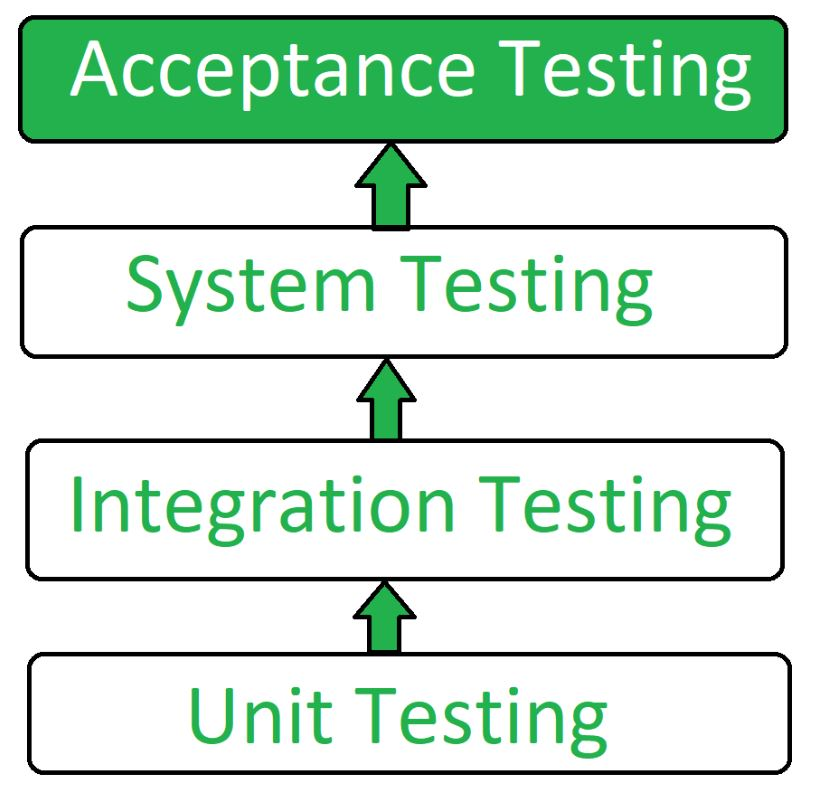
\includegraphics[width=0.5\textwidth]{Figures/test.jpg}
    \cite{web:acceptance}
\end{figure}
Estos \textit{teses} no son automáticos, sino que son realizados manualmente, realizando todas las acciones posibles y verificando que funcionan correctamente. Estos \textit{teses} se suelen realizar de igual manera que una lista de comprobación y que todos los \textit{checks} salgan correctos.
\begin{figure}[h!]
    \centering
    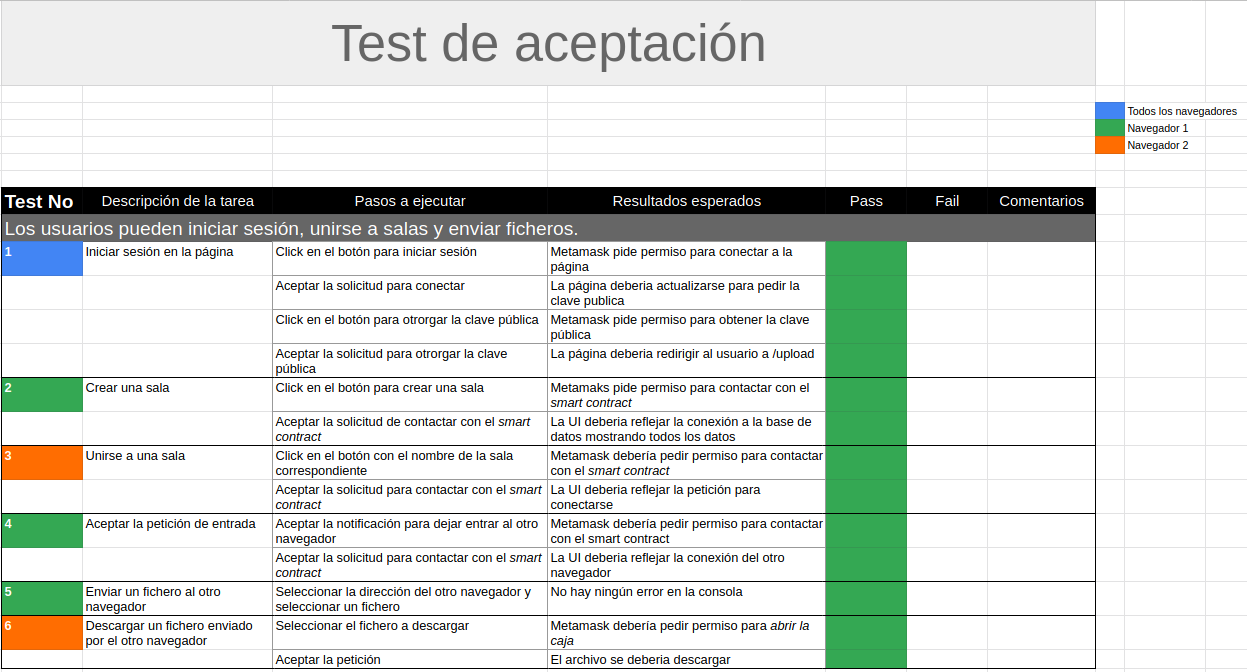
\includegraphics[width=1\textwidth]{Figures/test-superado.png}
    \caption{Imagen con tests de aceptación superados.}
    \label{fg:test}
\end{figure}
En este caso, es un \textit{tese} de aceptación que ha salido completamente satisfactorio \ref{fg:test}.
\subsection{Rendimiento}
A lo largo de este proyecto, se ha defendido la superioridad de implementar una aproximación distribuida al diseño ya que su uso permite una distribución del ancho de banda. Gracias a implementar una solución distribuida no es necesario enviar todos los datos; otros nodos pueden ayudar con el envío de datos. Aún así, para conocer mas de cerca IPFS, se va a comparar con FTP con la ayuda del trabajo "Performance Evaluation of IPFS in Private Networks" \cite{web:perf}. Este trabajo compara IPFS y FTP \cite{web:ftp} en rendimiento \textit{1to1}. Aunque los beneficios de IPFS se obtienen cuando existen más nodos, esto nos da luz en el rendimiento base. El trabajo compara el envío de ficheros grandes y pequeños. Considera un fichero pequeño entre (1kb - 256kb), en cambio, un fichero grande es considerado entre (1mb - 64mb).\\
\textbf{Latencia de escritura}\\
\begin{figure}[h!]
    \centering
    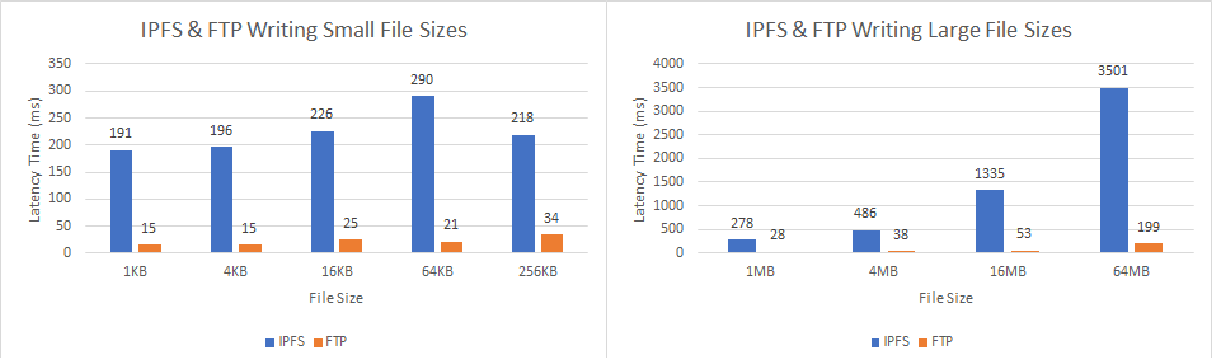
\includegraphics[width=1\textwidth]{Figures/4-Figure1-1.png}
    \caption{Figura con las latencias de escritura de IPFS y FTP}
    \label{fg:fig1}
\end{figure}
En la figura \ref{fg:fig1}, se puede ver que a la hora de hacer escrituras, IPFS tiene latencias superiores. Esto se debe a que FTP es un protocolo mucho más simple. FTP no hace ningún calculo para asegurar la legitimidad del fichero y de la red. En cambio IPFS si que tiene esta funcionalidad. Una vez más, se puede ver que IPFS está optimizado para ficheros pequeños.\\
\textbf{Latencia de lectura}\\
\begin{figure}
    \centering
    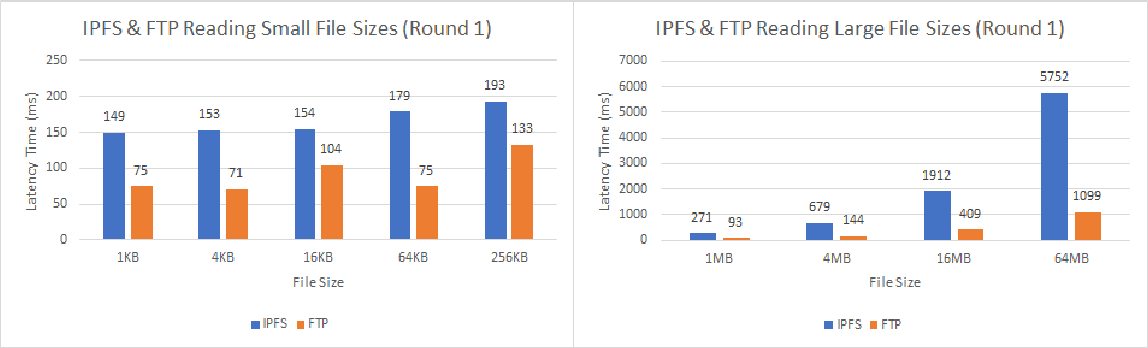
\includegraphics[width=1\textwidth]{Figures/4-Figure3-1.png}
    \caption{Figura con las latencias de lectura de IPFS y FTP}
    \label{fg:fig2}
\end{figure}
En esta figura \ref{fg:fig2}, se puede comprobar una velocidad superior por parte de FTP. Aún así, la diferencia de tiempos es inferior. Esto significa que si se tienen 17 \textit{peers} ( 16 tienen el fichero guardado y 1 lo solicita), podemos enviar un fichero de 64mb mientras cada \textit{peer} solo envía 4mb. De esta forma, el peer que solicita el fichero consigue obtenerlo mientras que el host original no tiene que preocuparse de enviar 64mb. Todo esto mientras utilizamos ligeramente menos porcentaje de CPU. Este proceso solo mejora cuando añadimos más nodos a la red. El uso de CPU es el punto débil de IPFS. Por eso mismo, uno de los objetivos principales de este proyecto ha sido disminuir el tamaño de los ficheros que se enviaban por la red. Es comprensible ya que FTP no gasta tiempo de ejecución realizando cálculos criptográficos para el envío de datos. FTP sin SFTP no utiliza encriptación de transporte.
\newpage
\thispagestyle{empty}